\problemname{Tycho}

\illustration{.4}{img/MarsPerseveranceRover.jpg}{}

\noindent
% The planetary exploration vehicle \emph{Tycho VIII} needs to get back to the home base after collecting mineral samples.
Pojazd do eksploracji planet \emph{Tycho VIII} musi wrócić do bazy macierzystej po zebraniu próbek minerałów.
% Tycho travels in a straight line from position~$0$ to the home base at position~$b$.
Tycho podróżuje w linii prostej z pozycji~$0$ do bazy domowej na pozycji~$b$.
% While moving, it advances at a slow but steady pace of $1$~unit per second.
Podczas ruchu posuwa się do przodu w wolnym, ale stałym tempie $1$~jednostki na sekundę.
% Every second, Tycho takes $1$~unit of environmental damage from the harsh planetary conditions.
W każdej sekundzie Tycho ponosi $1$~jednostkę szkód środowiskowych spowodowanych trudnymi warunkami panującymi na planecie.

% The situation is made even worse by radiation from a nearby pulsar, which adds $d$ additional units of damage every $p$ seconds.
Sytuację pogarsza jeszcze promieniowanie z pobliskiego pulsara, które dodaje $d$ dodatkowych jednostek obrażeń co $p$ sekund.
% However, the radiation damage can be avoided by seeking shelter in one of $n$ different hiding spots---caves, vegetation, large rocks, carcasses of the planet's megafauna---along the way.
Obrażeń od promieniowania można jednak uniknąć, szukając schronienia w jednej z $n$ różnych kryjówek --- jaskiniach, roślinności, dużych skałach, padlinach megafauny planety --- po drodze.
% Tycho can choose to stand still at any point for any integer number of seconds.
Tycho może zdecydować się na stanie w miejscu przez dowolną liczbę całkowitą sekund.

% The starting position~$0$ and the home base at~$b$ are both sheltered, so Tycho takes no radiation damage there.
Pozycja startowa~$0$ i baza domowa~$b$ są osłonięte, więc Tycho nie otrzymuje tam żadnych obrażeń od promieniowania.

\medskip
% What is the minumum damage Tycho will take on its journey back to the home base?
Jaka jest najmniejsza sumaryczna liczba obrażeń otrzymanych przez Tycho w drodze powrotnej do bazy?

\section*{Przykład}

% Consider the situation where the home base is at position $18$ and there are shelters at positions $8$ and $15$.
Rozważ sytuację, w której baza macierzysta znajduje się na pozycji $18$, a na pozycjach $8$ i $15$ znajdują się schrony.

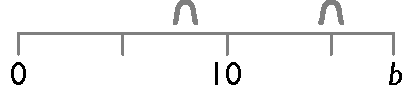
\includegraphics[width=.3\textwidth]{img/samplesetup}

% Assume that the pulsar's period is $4$, so unsheltered Tycho would take damage at times $4$, $8$, $12$, etc.
Przyjmij, że okres pulsara to $4$, więc Tycho poza schronieniem odbierałby obrażenia w momentach $4$, $8$, $12$, itd.
% If Tycho leaves from the starting position (where it's sheltered) at time $0$, it can reach the first shelter after $8$ seconds, incurring radiation damage $d$ at time $4$ (but none at time $8$ because it's sheltered then).
Jeśli Tycho wyjdzie z pozycji startowej (gdzie jest osłonięty) w czasie $0$, może dotrzeć do pierwszego schronu po $8$ sekundach, ponosząc obrażenia od promieniowania $d$ w czasie $4$ (ale żadnych w czasie $8$, ponieważ jest wtedy osłonięty).
% Continuing without stopping, it reaches the home base at time $18$, incurring $d+d$ more units of radiation damage (at times $12$ and $16$, respectively).
Kontynuując bez zatrzymywania się, dociera do bazy domowej w czasie $18$, ponosząc $d+d$ kolejnych jednostek obrażeń od promieniowania (odpowiednio w czasie $12$ i $16$).
% This way it incurs $d+d+d=3d$ units of radiation damage and $18$ units of environmental damage.
W ten sposób ponosi $d+d+d=3d$ jednostek obrażeń od promieniowania i $18$ jednostek obrażeń od środowiska.
% If instead Tycho waits at the $2$nd shelter (at position $15$) for $1$ second, the pulse at time $16$ causes it no damage, and it reaches the home base at time $19$ with a total of $2d + 19$ units of damage.
Jeśli zamiast tego Tycho czeka w schronie o numerze $2$ (na pozycji $15$) przez $1$ sekundę, impuls w czasie $16$ nie powoduje żadnych obrażeń, a do bazy macierzystej dociera w czasie $19$ z łączną liczbą $2d + 19$ jednostek obrażeń.
% This is better for most values of $d$.
Jest to lepsze rozwiązanie dla większości wartości $d$.
% The two situations are shown here:
Te dwie sytuacje są pokazane tutaj:

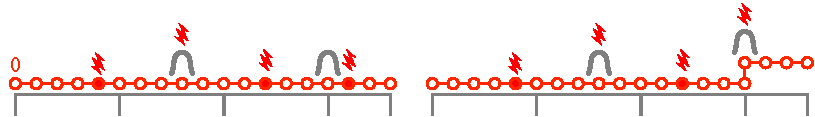
\includegraphics[width=.8\textwidth]{img/sample1_2.pdf}

% If the pulsar's period is $10$, Tycho can wait at the starting position for $2$~seconds and then just go home without stopping at any shelter.
Jeśli okres pulsara wynosi $10$, Tycho może czekać na pozycji startowej przez $2$~sekundy, a potem po prostu wrócić do domu, nie zatrzymując się w żadnym schronie.
% Thus it passes the $1$st shelter (at position~$8$) at just the right moment when the pulsar flares and arrives at the home base at time $20$, for a total of $20$ environmental damage and no radiation damage at all.
W ten sposób mija schron o numerze $1$ (na pozycji~$8$) we właściwym momencie, gdy pulsar rozbłyska i dociera do bazy macierzystej w czasie $20$, za łączną sumę $20$ szkód środowiskowych i żadnych szkód radiacyjnych.

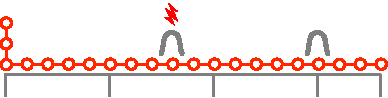
\includegraphics[width=.4\textwidth]{img/sample3.pdf}

\section*{Wejście}

% The first line consists of four integers $b$, $p$, $d$, and $n$, separated by single spaces:
Pierwsza linia składa się z czterech liczb całkowitych $b$, $p$, $d$, oraz $n$, oddzielonych pojedynczymi spacjami:
% the location $b$ of the home base,
lokalizacja $b$ bazy domowej,
% the pulsar's flare period~$p$,
okres rozbłysku pulsara~$p$,
% the additional radiation damage~$d$ caused by each flare of the pulsar,
dodatkowe szkody radiacyjne~$d$ spowodowane przez każdą flarę pulsara,
% the number~$n$ of the shelters.
liczba $n$ schronów.
% The following $n$~lines each contain an integer giving the shelter locations $a_1$, $\ldots$, $a_n$, with 
Kolejne $n$~wierszy zawierają po jednej liczbie całkowitej oznaczającej lokalizacje schronów $a_1$, $\ldots$, $a_n$, spełniające
$0<a_1<\cdots <a_n< b$. % constraint:shelterbounds, constraint:sortedshelters

\section*{Wyjście}

% Print a single integer: the minimum amount of damage Tycho must take to reach $b$.
Wypisz pojedynczą liczbę całkowitą: minimalną ilość obrażeń, jakie musi przyjąć Tycho, by dotrzeć na pozycję~$b$.

\section*{Ograniczenia i punktacja}

% You can assume
Możesz założyć
$p < b$ % constraint:pulsehappens
% and
oraz
$n < b$. % constraint:sheltersfit
% We always have
Zawsze jest spełnione
$1\leq b\leq 10^{12}$, % constraint:b
$0\leq d \leq 10^6$, %constraint:d
% and
oraz
$0\leq n \leq 10^5$. % constraint:n

% Your solution will be tested on a set of test groups, each worth a number of points.
Twoje rozwiązanie zostanie przetestowane na zestawie grup testowych, z których każda jest warta pewną liczbę punktów.
% Each test group contains a set of test cases.
Każda grupa testowa zawiera zestaw przypadków testowych.
% To get the points for a test group you need to solve all test cases in the test group.
Aby uzyskać punkty za grupę testową musisz rozwiązać wszystkie przypadki testowe w tej grupie.
% Your final score will be the maximum score of a single submission.
Twój ostateczny wynik będzie maksymalnym wynikiem pojedynczego zgłoszenia.

\medskip
\begin{tabular}{lll}
% Group & Points & Constraints \\\hline
Grupa & Punkty & Ograniczenia \\\hline
%   $1$ & $8$  & $p\leq 10^6$ and Tycho does not need to wait \emph{after} leaving position~$0$.$^*$ \\ % constraint:nowait
  $1$ & $8$  & $p\leq 10^6$ oraz Tycho nie musi czekać \emph{po} wyjściu z pozycji~$0$.$^*$ \\ % constraint:nowait
  $2$ & $5$  & $b\leq 1000$, $p\leq 100$, $n\leq 10$ \\
  $3$ & $7$  & $b\leq 1000$ \\
  $4$ & $15$ & $p\leq 10^6$, $n\leq 1000$\\
  $5$ & $20$ & $p\leq 100$\\
  $6$ & $35$ & $p\leq 10^6$\\
%   $7$ & $10$ & \emph{No additional constraints}
  $7$ & $10$ & \emph{Brak dodatkowych ograniczeń}
\end{tabular}

\medskip
% \noindent $^*$ In test group~$1$, Tycho may still need to wait at position~$0$ \emph{before} it starts moving.
\noindent $^*$ W grupie testowej~$1$, Tycho może nadal potrzebować czekać na pozycji~$0$ \emph{zanim} zacznie się poruszać.
% For example, sample inputs $2$, $3$, and $4$ belong to test group~$1$.
Na przykład, przykładowe wejścia $2$, $3$, oraz $4$ należą do grupy testowej~$1$.
